% Requires in preamble:
% \usepackage{pgfplots}
% \pgfplotsset{compat=1.18}
% \usetikzlibrary{arrows.meta}

\definecolor{cblue}{RGB}{0, 85, 150}
\definecolor{cvermilion}{RGB}{215, 85, 0}
\definecolor{cpurple}{RGB}{115, 50, 130}

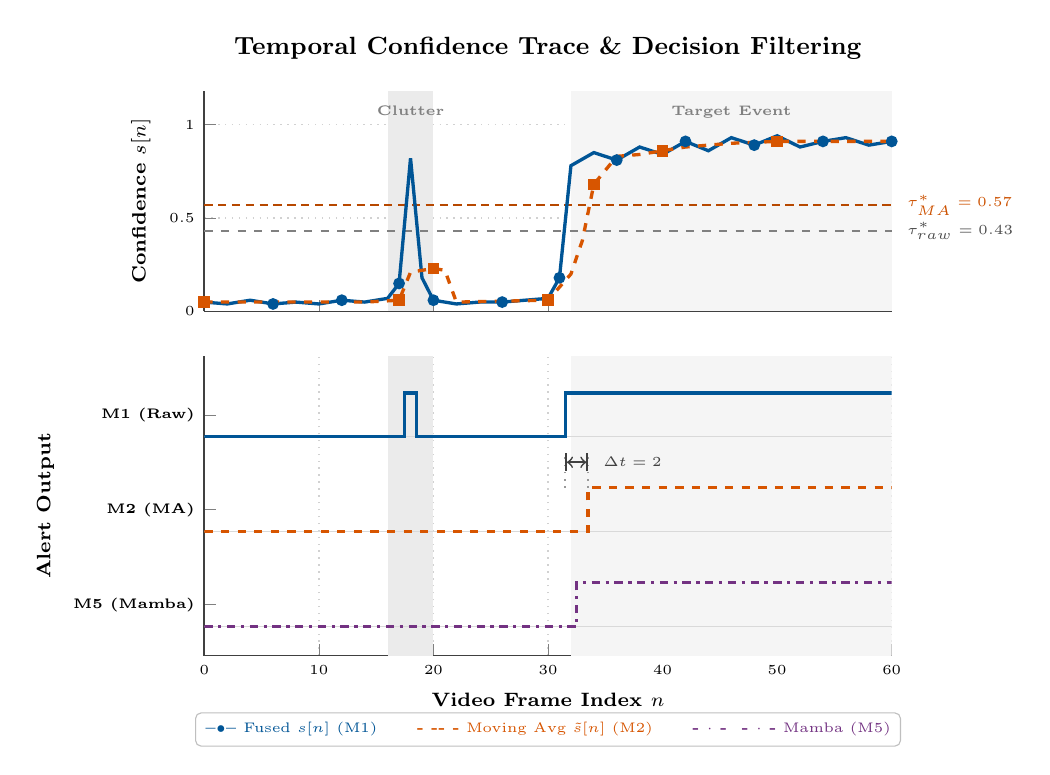
\begin{tikzpicture}
  \pgfplotsset{
    scale only axis,
    width=0.72\columnwidth, % Sized to reserve gutter space for right-side threshold labels
    xmin=0,
    xmax=60,
    tick label style={font=\tiny},
    axis line style={semithick, black!75},
    grid style={dotted, black!18, line width=0.5pt},
  }
%
  % -------------------------------------------------------------
  % TOP PANEL: Fused Confidence & Filter Responses
  % -------------------------------------------------------------
  \begin{axis}[
    name=top_axis,
    clip=false, % Allows labels at x=60 to render outside the plot frame
    title={\small\textbf{Temporal Confidence Trace \& Decision Filtering}},
    title style={yshift=2pt},
    height=2.8cm,
    ymin=0,
    ymax=1.18,
    ytick={0.0, 0.5, 1.0},
    ymajorgrids=true,
    ylabel={Confidence $s[n]$},
    ylabel style={font=\scriptsize\bfseries},
    xtick={0, 10, 20, 30, 40, 50, 60},
    xticklabels=\empty,
    axis x line*=bottom,
    axis y line*=left,
  ]
    % Background Intervals
    \fill[black!8] (axis cs:16, 0) rectangle (axis cs:20, 1.18);
    \node[font=\tiny\bfseries, text=black!50, anchor=north] at (axis cs:18, 1.15) {Clutter};

    \fill[black!4] (axis cs:32, 0) rectangle (axis cs:60, 1.18);
    \node[font=\tiny\bfseries, text=black!50, anchor=north] at (axis cs:46, 1.15) {Target Event};

    % Threshold Lines (Labels placed directly to the right of each dashed line)
    \draw[dash pattern=on 3pt off 2pt, draw=cvermilion!85!black, line width=0.7pt] 
      (axis cs:0, 0.57) -- (axis cs:60, 0.57)
      node[right=2pt, font=\tiny\bfseries, text=cvermilion!95!black] {$\tau_{\text{MA}}^* = 0.57$};

    \draw[dashed, draw=black!50, line width=0.6pt] 
      (axis cs:0, 0.43) -- (axis cs:60, 0.43)
      node[right=2pt, font=\tiny\bfseries, text=black!70] {$\tau_{\text{raw}}^* = 0.43$};

    % Trace 1: Fused raw confidence s[n]
    \addplot[
      color=cblue,
      very thick,
      solid,
      mark=*,
      mark repeat=3,
      mark options={scale=0.75, fill=cblue}
    ] coordinates {
      (0, 0.05)  (2, 0.04)  (4, 0.06)  (6, 0.04)  (8, 0.05)
      (10, 0.04) (12, 0.06) (14, 0.05) (16, 0.07) (17, 0.15)
      (18, 0.82) (19, 0.18) (20, 0.06) (22, 0.04) (24, 0.05)
      (26, 0.05) (28, 0.06) (30, 0.07) (31, 0.18) (32, 0.78)
      (34, 0.85) (36, 0.81) (38, 0.88) (40, 0.84) (42, 0.91)
      (44, 0.86) (46, 0.93) (48, 0.89) (50, 0.94) (52, 0.88)
      (54, 0.91) (56, 0.93) (58, 0.89) (60, 0.91)
    };

    % Trace 2: Moving average s_MA[n]
    \addplot[
      color=cvermilion,
      very thick,
      dashed,
      mark=square*,
      mark repeat=3,
      mark options={scale=0.75, fill=cvermilion, solid}
    ] coordinates {
      (0, 0.05)  (8, 0.05)  (14, 0.05) (17, 0.06) (18, 0.21)
      (19, 0.22) (20, 0.23) (21, 0.22) (22, 0.05) (30, 0.06)
      (32, 0.20) (33, 0.38) (34, 0.68) (36, 0.83) (38, 0.84)
      (40, 0.86) (42, 0.88) (46, 0.90) (50, 0.91) (54, 0.91)
      (60, 0.91)
    };
  \end{axis}
%
  % -------------------------------------------------------------
  % BOTTOM PANEL: Alert Waveforms with Expanded Row Padding
  % -------------------------------------------------------------
  \begin{axis}[
    name=bottom_axis,
    at=(top_axis.below south west),
    anchor=above north west,
    yshift=-0.32cm,
    height=3.8cm,
    ymin=-0.2,
    ymax=3.9,
    ytick={0.5, 1.8, 3.1},
    yticklabels={%
      {\bfseries M5 (Mamba)},
      {\bfseries M2 (MA)},
      {\bfseries M1 (Raw)}%
    },
    ylabel={Alert Output},
    ylabel style={font=\scriptsize\bfseries},
    yticklabel style={font=\tiny},
    ymajorgrids=false,
    xmajorgrids=true,
    xtick={0, 10, 20, 30, 40, 50, 60},
    xlabel={Video Frame Index $n$},
    xlabel style={font=\scriptsize\bfseries},
    axis x line*=bottom,
    axis y line*=left,
  ]
    % Aligned Intervals
    \fill[black!8] (axis cs:16, -0.2) rectangle (axis cs:20, 3.9);
    \fill[black!4] (axis cs:32, -0.2) rectangle (axis cs:60, 3.9);

    % Baseline Reference Rails (0-state)
    \draw[black!15, line width=0.5pt] (axis cs:0, 2.8) -- (axis cs:60, 2.8);
    \draw[black!15, line width=0.5pt] (axis cs:0, 1.5) -- (axis cs:60, 1.5);
    \draw[black!15, line width=0.5pt] (axis cs:0, 0.2) -- (axis cs:60, 0.2);

    % M1 (Raw): Spurious pulse at frame 18; onset at frame 31.5
    \addplot[color=cblue, very thick, const plot] coordinates {
      (0, 2.8) (17.5, 3.4) (18.5, 2.8) (31.5, 3.4) (60, 3.4)
    };

    % M2 (MA): Suppressed spike; onset at frame 33.5
    \addplot[color=cvermilion, very thick, dashed, const plot] coordinates {
      (0, 1.5) (33.5, 2.1) (60, 2.1)
    };

    % M5 (Mamba): Suppressed spike; onset at frame 32.5
    \addplot[color=cpurple, very thick, dashdotted, const plot] coordinates {
      (0, 0.2) (32.5, 0.8) (60, 0.8)
    };

    % Clean Latency Measurement
    \draw[dotted, black!40, semithick] (axis cs:31.5, 2.1) -- (axis cs:31.5, 2.55);
    \draw[dotted, black!40, semithick] (axis cs:33.5, 2.1) -- (axis cs:33.5, 2.55);
    \draw[|<->|, semithick, black!75] (axis cs:31.5, 2.45) -- (axis cs:33.5, 2.45);
    \node[anchor=west, font=\tiny\bfseries, text=black!75] at (axis cs:34.0, 2.45) {$\Delta t = 2$};
  \end{axis}
%
  % -------------------------------------------------------------
  % COLOR LEGEND: Centered Below the Bottom X-Axis
  % -------------------------------------------------------------
  \node[
    anchor=north,
    yshift=-0.72cm,
    draw=black!25,
    fill=white,
    rounded corners=2pt,
    font=\tiny,
    inner sep=3.5pt
  ] at (bottom_axis.south) {
    \textcolor{cblue}{\textbf{--$\bullet$--} Fused $s[n]$ (M1)} \hspace{1.4em}
    \textcolor{cvermilion}{\textbf{- -$\blacksquare$- -} Moving Avg $\tilde{s}[n]$ (M2)} \hspace{1.4em}
    \textcolor{cpurple}{\textbf{- $\cdot$ - $\blacktriangle$ - $\cdot$ -} Mamba (M5)}
  };
\end{tikzpicture}